\chapter{Comparative study of visual explanation systems for item recommendation}\label{chapter:survey}



Tintarev and Masthoff give a number of objectives for explanation systems. The following listing is adapted from \cite{tintarev:2007:SER:1547550.1547664}:

\begin{itemize}
	\item \textbf{Transparency}: explain how the system works;
	\item \textbf{Scrutability}: allow users to tell;
	\item \textbf{Trust}: increase users' confidence in the system;
	\item \textbf{Effectiveness}: help users make good decisions;
	\item \textbf{Persuasiveness}: convince users to try or buy;
	\item \textbf{Efficiency}: help users make decisions faster;
	\item \textbf{Satisfaction}: increase the ease of usability or enjoyment.
\end{itemize}

\section{Applications}\label{chapter:survey:section:applications}

\subsection{Smallworlds}\label{chapter:survey:section:applications:subsection:smallwords}

In \cite{gretarsson:2010}, Gretarsson et al. used the Facebook API to create an application to generate social recommendations for Facebook users. Unfortunately the Facebook API does not support unauthorized reading of item preference information beyond the immediate friend group. This would not have been a problem unless traditional collaborative filtering strategies tend to produce item suggestions of inferior quality for small items. In this case however the research team relies on the social filtering through the active user's peer group\cite{gretarsson:2010}.

\emph{SmallWorlds}\index{SmallWorlds} is "a visual interactive graph-based interface that allows users to specify, refine and build item-preference profiles"\cite{gretarsson:2010}. The system promotes transparancy in the recommendation process, and gives the user a sense of control over the recommendation process through interactions. This way, Gretarsson et al. try to further overcome the limitations of their recommender system\cite{gretarsson:2010}.

SmallWorlds uses a five-layered design to create suggestions:

\begin{enumerate}
	\item the active user's node;
	\item the active user's profile items;
	\item friends who have items in common with the active user;
	\item items that are not in the active user’s profile, but are liked by friends in layer $3$;
	\item friends who have no items in common with the active user and items in their profiles, but not items in the profiles of friends in layer $3$.
\end{enumerate}

The user can move nodes in each layer further or closer towards the active user's node to adjust the weights of each node. This is used in combination with similarity functions to calculate the suggestions. Figure \ref{figure:smallworlds} shows a screenshot of the application.

\begin{figure}%
	\begin{center}
		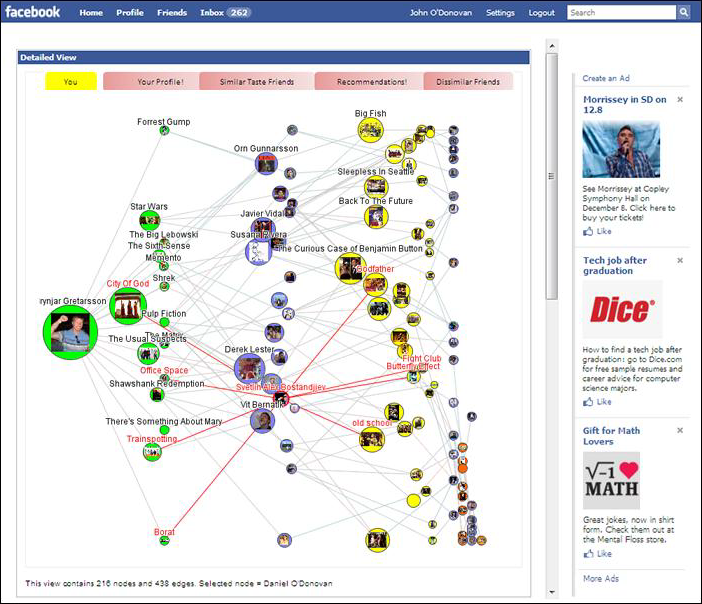
\includegraphics[width=350px]{img/smallworlds}%
	\end{center}
	\caption{The SmallWords interface.}%
	\label{figure:smallworlds}%
\end{figure}


\subsection{Pharos}\label{chapter:survey:section:applications:subsection:pharos}

Content-centric social websites, such as blogs and discussion forums, contain vast amounts of fast growing information. Recommendation systems have been developed to help users find the information they are looking for. The \emph{Pharos}\index{Pharos} application tries to address two distinctive problems that present themselves in this context: the cold start problem and the black box problem\cite{zhao:2010}, as described earlier in section \ref{chapter:literature_study:section:computer:subsection:challenges}.

As they hope to overcome previously defined problems, Zhao et al. \cite{zhao:2010} collect and visualize content-related social behaviour. The resulting data set is tranformed into a social map. The social map provides a context for new users, addressing the cold start problem. Secondly, the user can explore the social map to increase understanding and user interaction, in an effort to overcome the black box problem.

The generation of the social map takes place through the following three step process:

\begin{itemize}
	\item \textbf{Community extraction}: a map depicting 'which users are talking about what'. Starting from either relationships, people or content communities can be derived;
	\item \textbf{Community/item/people ranking}: the next step is to rank these communities. The 'hotness' can be measured on content, people authorities and so on;
	\item \textbf{Community labeling}: describing what each community is about.
\end{itemize}

An example of what the resulting visualization looks like, is depicted in figure \ref{figure:pharos}.

\begin{figure}%
	\begin{center}
		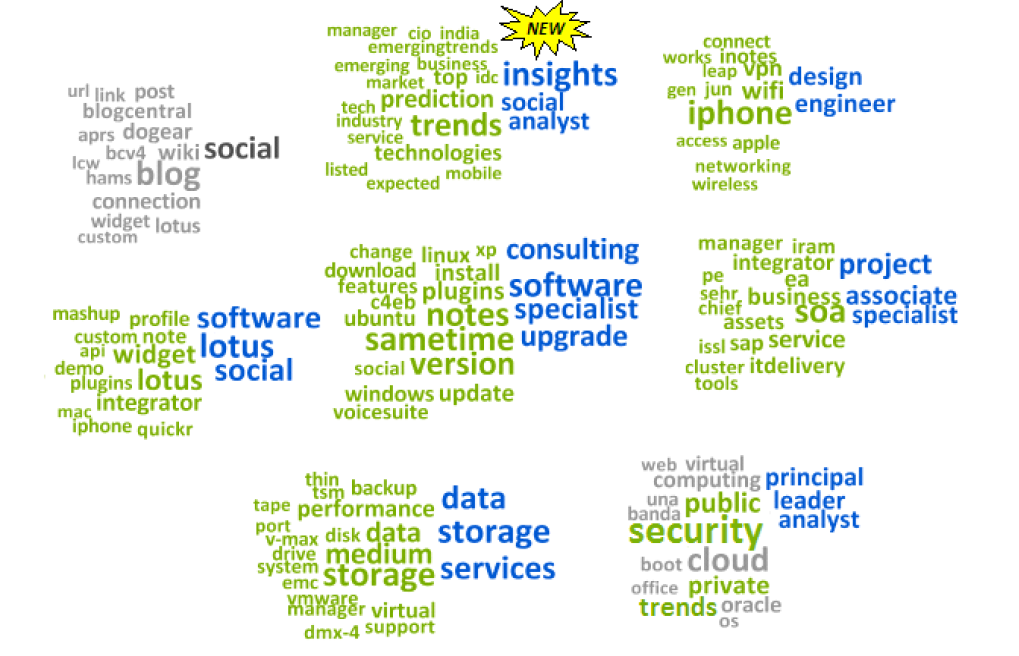
\includegraphics[width=350px]{img/pharos}%
	\end{center}
	\caption{The Pharos social map. Colours indicate activity within a certain group.}%
	\label{figure:pharos}%
\end{figure}


\subsection{TasteWeights}\label{chapter:survey:section:applications:subsection:tasteweights}

Social web APIs and other data sources are constantly evolving, and traditional recommender system techniques such as automated collaborative filtering need to adapt to the changing environment of the social web (cf. Smallworlds).

Bostandjiev et al. introduces two enhancements for the traditional techniques. Multiple web sources, namely from Facebook, Twitter and Wikipedia are combined when computing the recommendation. This combination provides a hybrid of different recommendation strategies, namely: collaborative filtering, expert-based and content-based respectively. The other feature is a new user interface that provides transparency into the recommendation process. The TasteWeights application uses this approach.

There are three levels to be distinguished that are represented visually as well:

A profile layer: liked items on Facebook,
A context layer: items coming from different sources,
A recommendation layer containing the actual recommendations.
Nodes of a graph reside in one of these layers. The user can influence the outcome of the recommendation by attributing weights to the nodes in the profile layer and context layer.

\begin{figure}%
	\begin{center}
		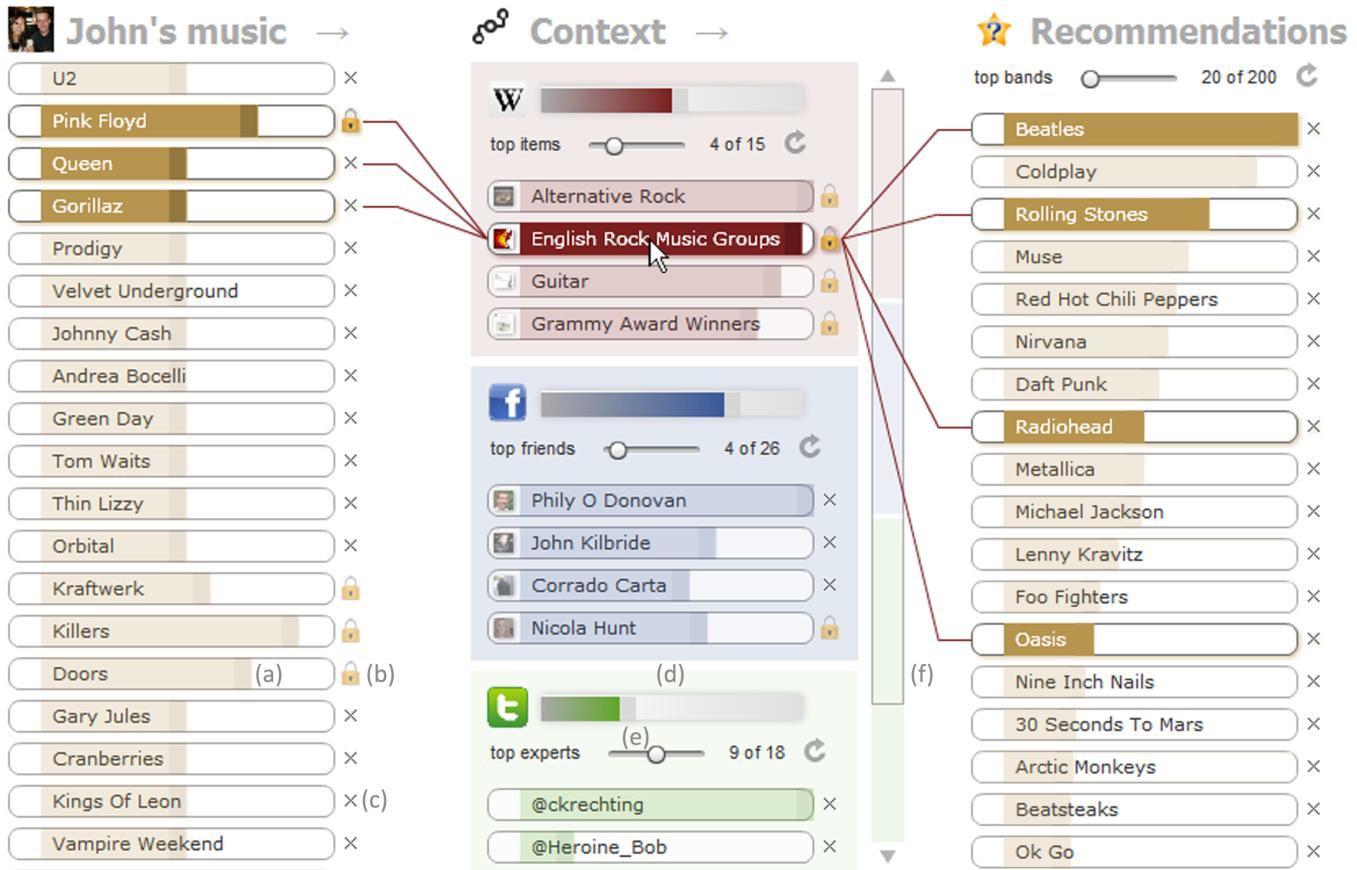
\includegraphics[width=350px]{img/tasteweights}%
	\end{center}
	\caption{The TasteWeights interface.}%
	\label{figure:tasteweights}%
\end{figure}


\subsection{SFVis}\label{chapter:survey:section:applications:subsection:sfvis}

SFVis (Social Friends Visualization) is an application that helps users explore and find friends interactively under a context of interest. The system is a hybrid approach of social tags and social networks. The SFVis framework transforms a data model (social tags and social networks) into a visual form. Users can both manipulate the input and visuals on demand.

Social tags can form a network. Within this structure clusters may arise. From this cluster tag network a hierarchy is derived. A compound graph is generated from the tag hierarchy and social networks.

A mapping function assigns actors in a social network to a tag tree. The actor similarity algorithm in SFVis considers both structure similarity in a social network and semantic similarity in a tag network. These scores will allow the recommendation system to compute friend suggestions.

SFVis uses circular visualizations for the different trees and graphs for both views as well as interaction with the user.


\subsection{PeerChooser}\label{chapter:survey:section:applications:subsection:peerchooser}

Due to black-box nature of collaborative filtering O’Donovan introduces PeerChooser. This system provides visual explanations for collaborative filtering recommendations and enables users to manipulate their neighborhood at varying levels of granularity.

This way the researchers hope to overcome the so-called grey-sheep problem. This occurs when a user’s history does not help to identify a set of similar recommendation partners.

\begin{figure}%
	\begin{center}
		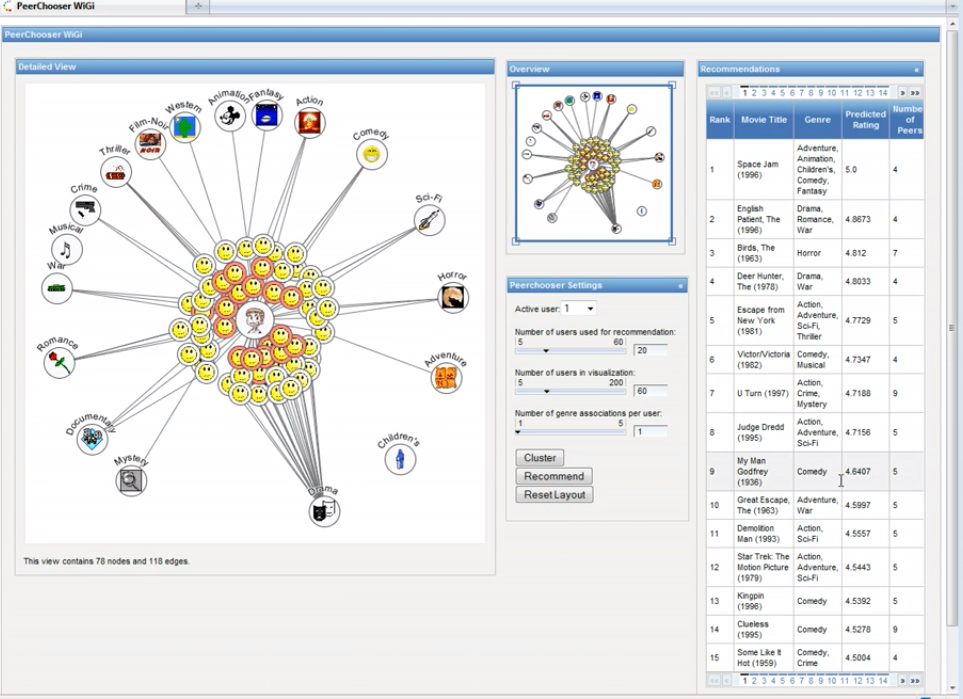
\includegraphics[width=350px]{img/peerchooser}%
	\end{center}
	\caption{The PeerChooser interface.}%
	\label{figure:peerchooser}%
\end{figure}


\section{Comparison overview}\label{chapter:survey:section:overview}


Table1 : overview recommender system case studies
In table 1 an overview is presented of some the different recommender systems and some of their properties. So far most of the applications discussed here used collaborative filtering and some kind of visualization and allowed the user to interact with the system.